\chapter{Introdução\label{chap:Introducao}}

O mercado global de animação e jogos foi avaliado em \$122.20 bilhões em 2010 e
é esperado que esta cifra atinja  \$242.93 bilhões em 2016. Esse mercado global
pode ser dividido em mercados específicos voltados para a Educação, o
Desenvolvimento para Web e a Animação para Entretenimento, podendo esse último
ser ainda subdividido em várias categorias \cite{animationMarketSize}, sendo
\textbf{Filmes} e \textbf{Efeitos Visuais} categorias de especial interesse para
este trabalho. 

Uma tarefa recorrente dentro da indústria cinematográfica é a modelagem e
animação de objetos tridimensionais. Tais objetos não estão sujeitos às
restrições do mundo físico e permitem gerar cenas e movimentos dificilmente
filmados de outra forma. Mesmo em produções com atores reais as técnicas de
Animação Computacional se fazem presentes, seja transformando o cenário do
filme, projetando sobre o ator uma textura que modifica suas feições ou
adicionando à obra um personagem completamente digital. Presentes em
praticamente qualquer novo \textit{blockbuster}, as técnicas de animação
tridimensional ainda apresentam custos elevados e proibitivos para certas
aplicações.

O orçamento para a produção de um filme inclui custos de pré-produção, filmagem,
pós-produção e divulgação, devendo-se levar em conta os direitos pelo roteiro,
salários dos atores, salários da equipe de produção, construção do set de
filmagens, efeitos especiais, figurino e tudo o mais \cite{movieProductionCost}.
Apesar da Animação Computacional diminuir o custo de alguns dos componentes
citados, ela é em si uma técnica cara. Dessa forma, ao passo que a animação
computacional  reduz custos com montagem de cenários e até mesmo maquiagem,
muitas vezes um único quadro de um filme pode requerer a animação de milhões de
partes móveis. No filme \textit{Monstros SA (2001)}, por exemplo, foram
utilizados mais de 2 milhões de fios de cabelo individualmente nomeados para a
construção do personagem Sully. Um único quadro com o personagem custou em média
de 11 a 12 horas de trabalho criativo \cite{sullyExample}. Com tantas horas de
trabalho criativo gastas durante o processo de animação, é evidente a
necessidade do desenvolvimento de técnicas que auxiliem os animadores.

Uma técnica importante que vem ao auxílio dos animadores consiste em transferir
movimentos e expressões de um ator para um modelo computacional. Metodologias
para captura ótica de performance teatral capazes de registrar expressões de um
ator em geometria detalhada são utilizadas na indústria já há algum tempo.
Exemplo conhecido do uso dessa tecnologia é o personagem \textit{Gollum} no
filme \textit{O Senhor dos Anéis: A Sociedade do Anel } (2001), onde o ator Andy
Serkis utiliza uma roupa especial com marcadores visuais durante as gravações
para que mais tarde a equipe de efeitos visuais renderize sobre ele um modelo
computacional tridimensional da criatura amaldiçoada. Mais recentemente, a mesma
tecnologia - em estado aprimorado e muito mais rica em detalhes - é utilizada em
\textit{O hobbit} (2015), onde o ator Benedict Cumberbatch dá vida ao dragão
Smaug. A Figura \ref{fig:smaug} ilustra o processo. Na Figura \ref{fig:smaugA}
observa-se o modelo que está sendo animado pela performance do ator. Na Figura
\ref{fig:smaugB} mostra-se em detalhes pontos colocados no rosto do ator para
auxiliar a captura de expressões. 

\begin{figure*}[!htb]
   \centering
 \begin{subfigure}[]{\label{fig:smaugA}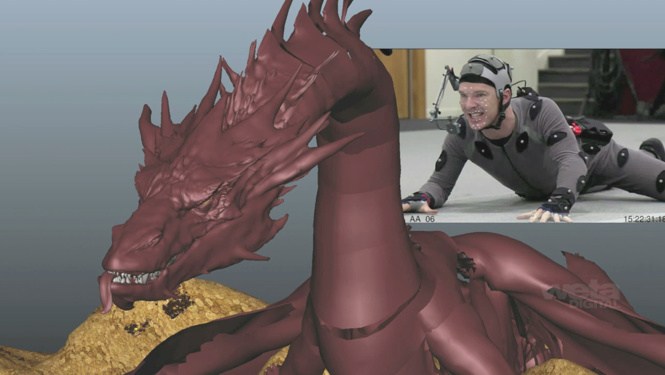
\includegraphics[width=0.4\linewidth]{./figs/exemploSmaug.jpg}}
  \end{subfigure}   
   \begin{subfigure}[]{\label{fig:smaugB}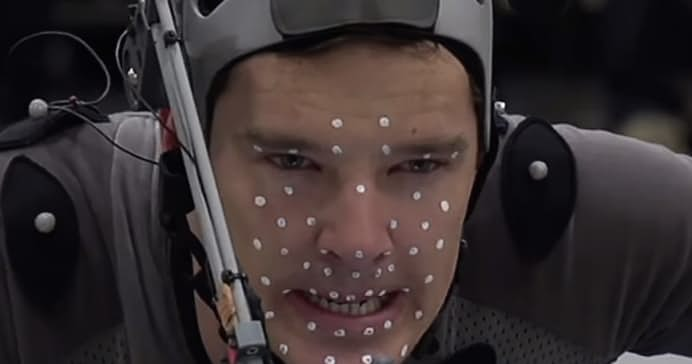
\includegraphics[width=0.4\linewidth]{./figs/Smaug_Benedict.jpg}}
  \end{subfigure}   
    \caption{Exemplo de utilização de captura de movimentos e expressões 
    na indústria cinematográfica. Pontos cuidadosamente colocados no rosto
  do ator são utilizados para transferir expressões para o modelo 
  tridimensional do personagem (retirado de \cite{sherlocksmaug}).}
    \label{fig:smaug}
\end{figure*}

Nesse tipo de aplicação cinematográfica requer-se do sistema de animação
computacional uma alta precisão no ajuste do modelo computacional ao ator em
cena. Para esse fim, utilizam-se ambientes especiais de filmagem , iluminação
controlada e marcadores visuais, sendo que muitas vezes a captura da imagem é
feita por um arranjo de câmeras ou ainda por câmeras de alta resolução. Além
disso, o resultado do processamento recebe um ajuste fino realizado por vários
artistas para que o resultado apresentado seja o mais convincente possível. Vale
notar que não é possível realizar esse ajuste fino caso não haja um longo prazo
disponível entre a captura da imagem e o instante em que os resultados precisam
ser apresentados ao público.

Uma outra utilização das técnicas de animação auxiliada por captura de vídeo é a
produção de shows com fantoches digitais.  Nesse espetáculo do entretenimento,
visto em programas televisivos e em parques de diversão ao redor do mundo, uma
equipe em uma câmara escondida anima em tempo real um modelo projetado em tela e
responde ao vivo às perguntas do público. O personagem animado apresenta
expressões corporais e faciais que encantam o público, deixando os mais novos
convencidos de que conversaram com seu personagem preferido e os mais velhos se
perguntando como aquilo pode ser possível. Vale observar que nesse caso os
requisitos de tempo são muito mais severos, uma vez que o resultado da animação
computacional deve ser apresentado rapidamente ao usuário para que a interação
entre público e personagem digital aconteça de forma dinâmica. Com isso em
mente, não é possível o ajuste fino de uma equipe de artistas, mas ainda sim é
possível fazer uso de iluminação controlada, câmera(s) de alta qualidade,
marcadores visuais. A equipe por trás do personagem pode ainda fazer uso de
controles pré-programados.

Apesar da tecnologia existente apresentar resultados adequados para as
aplicações citadas, ela apresenta um custo elevado. Dessa forma, ainda que
grandes empresas se disponham a bancar o preço da tecnologia atual, os custos
com software, hardware e com a equipe técnica envolvida podem dificultar a
utilização de técnicas de animação computacional em produtos desenvolvidos por
empresas de recursos mais modestos.  Portanto, o desenvolvimento de produtos que
realizem as mesmas tarefas a custos mais baixos é certamente de interesse do
mercado de animação. Tal produto poderia, por exemplo, ser utilizado por
desenvolvedores de animações independentes para acelerar e baratear seus
projetos.  

Um exemplo de animações de baixo orçamento pode ser encontrado na produção de
programas televisivos infantis cujo objetivo seja trabalhar uma temática de
interesse social ou atingir um público que não o público geral. Por exemplo, um
nicho de crianças comumente não atendido pelas opções de programas infantis é o
de crianças autistas. Apesar das dificuldades encontradas por essas crianças
variarem muito de um indivíduo para o outro, é comum que crianças autistas
apresentem dificuldade em manter contato visual, mesmo que seja com personagens
de um filme. Tal fato não é levado em consideração por animações convencionais,
o que as torna inadequadas para serem assistidas por crianças com a dificuldade
citada. Tendo em vista que animações infantis podem ser utilizadas como uma
importante ferramenta educacional, há certamente motivação para o
desenvolvimento de desenhos infantis próprios para as crianças autistas.

Uma empresa interessada em desenvolver tais animações muito provavelmente tem o
objetivo de atender a um interesse social acima do objetivo de atender fins
lucrativos.  Consequentemente, a equipe dificilmente terá os mesmos recursos
financeiros de uma que trabalhe com o público geral e poderá enfrentar
dificuldades em arcar com os custos envolvidos.  Objetiva-se com esse trabalho
que o produto desenvolvido possa ser utilizado como ferramenta para auxiliar o
desenvolvimento de programas infantis com foco em crianças autistas.

Colocando de forma clara, o objetivo desse trabalho é desenvolver um sistema de
animação auxiliada por captura de vídeo que seja capaz de transferir expressões
faciais do usuário para uma avatar computacional. Além disso, o sistema não deve
requirir nenhuma estrutura elaborada: ele deve rodar em hardware comum e ser
robusto à iluminação, ruídos presentes no processo de captura de imagem e não
deve utilizar marcadores visuais.  A intenção é que o sistema funcione em uma
máquina de configurações acessíveis e utilize câmeras de qualidade comparável à
\textit{webcams} comumente encontradas em computadores pessoais.


O Capítulo 2 deste trabalho trata da fundamentação teórica por trás das técnicas
utilizadas. Reconhecimento de pontos do rosto, renderização de objetos
tridimensionais, filtragem digital e estimação de profundidade são tópicos
abordados. No Capítulo 3 as técnicas introduzidas são relacionados para compor a
metodologia do sistema proposto neste trabalho.  No Capítulo 4 os resultados
obtidos são apresentados e discutidos.  O último capítulo elabora conclusões e
aponta propostas de melhorias futuras para o sistema de auxílio a animação
computacional desenvolvido.
